% =============================================================================
% NO2 en España — paper técnico
% Compilar:  latexmk -pdf paper.tex     (o make)
% =============================================================================
\documentclass[10pt,twocolumn,a4paper]{article}

\usepackage[utf8]{inputenc}
\usepackage[T1]{fontenc}
\usepackage[spanish,es-noquoting]{babel}
\usepackage[margin=2cm,columnsep=6mm]{geometry}
\usepackage{amsmath,amssymb}
\usepackage{graphicx}
\usepackage{booktabs}
\usepackage{siunitx}
\usepackage{lmodern}
\usepackage{microtype}
\usepackage[font=small,labelfont=bf]{caption}
\usepackage{natbib}
\usepackage[hidelinks]{hyperref}
\usepackage{xcolor}
\usepackage{authblk}

\sisetup{output-decimal-marker={,}, group-separator={\,}}
\newcommand{\ugm}{\si{\micro\gram\per\cubic\metre}}
\newcommand{\nodos}{\ce{NO2}}
\usepackage[version=4]{mhchem}

\bibliographystyle{apalike}
\setlength{\bibsep}{2pt}

\title{\bfseries La escala importa: convergencia entre el agrupamiento de
fuentes industriales y su influencia sobre el \ce{NO2} de fondo en España}

\author[ ]{Randy Fernández}
\affil[ ]{\small Máster en Ciencia de Datos \\
\texttt{randy.fernandez@example.com}}
\date{}

\begin{document}
\maketitle

% =============================================================================
\begin{abstract}
\noindent
La atribución del \ce{NO2} de fondo a fuentes industriales o a urbanización
está mal condicionada en la mayoría de los países europeos porque ambos
factores son espacialmente colineales. España constituye una excepción: sus
grandes focos industriales están desacoplados de los focos urbanos.
Explotamos esa separación para estimar, mediante tres ramas metodológicas
independientes, a qué escala espacial opera la influencia industrial sobre la
concentración de fondo. Un proceso de conglomerados de Thomas ajustado
únicamente a las coordenadas de \num{297} instalaciones E-PRTR estima un
diámetro efectivo del distrito industrial de \SI{10.7}{\kilo\metre}; un
barrido independiente de anchos de banda que acopla la intensidad de emisión
con las concentraciones observadas en \num{212} estaciones de fondo sitúa la
escala óptima de influencia en \SI{10.0}{\kilo\metre} ($F=13{,}86$,
$p=\num{2.5e-4}$). La razón entre ambas es \num{0.93}. Ninguna de las dos
estimaciones utiliza la información de la otra. A escala provincial
(\textsc{nuts}-3, $n=50$) el efecto industrial desaparece por completo y
resiste cuatro intentos de refutación, incluidas \num{1000} zonificaciones
alternativas en las que resulta significativo solo el \SI{2.5}{\percent} de
las veces. Mostramos que la desaparición no es falta de potencia sino un
efecto de la unidad de análisis: un radio de influencia de
\SI{10}{\kilo\metre} cubre el \SI{0.8}{\percent} de la provincia media
española. Derivamos una cota superior para el efecto industrial areal de
\SI{0.96}{\ugm} ---el \SI{22.3}{\percent} de la media nacional de fondo---
frente a un recargo local de tráfico de aproximadamente \SI{3.5}{\ugm}.

\medskip
\noindent\textbf{Palabras clave:} geoestadística, procesos puntuales, MAUP,
cambio de soporte, calidad del aire, \ce{NO2}.
\end{abstract}

% =============================================================================
\section{Introducción}

El dióxido de nitrógeno es, entre los contaminantes regulados, aquel en que la
pregunta ``¿industria o tráfico?'' permanece genuinamente abierta a escala
regional. A diferencia del material particulado, dominado por fuentes difusas
y transporte de largo alcance, el \ce{NO2} tiene una firma doble: emisiones
puntuales de gran magnitud procedentes de instalaciones industriales de
combustión, y emisiones lineales difusas asociadas al tráfico rodado. Los
modelos empíricos de calidad del aire de referencia
---\emph{land use regression} y sus variantes de aprendizaje
automático \citep{beelen2013,chen2019,vizcaino2018}--- alcanzan capacidades
predictivas notables ($R^2$ entre \num{0.5} y \num{0.8}) pero no separan
mecanismos: sus covariables de uso del suelo capturan simultáneamente
urbanización, industria y transporte porque en la mayoría del territorio
europeo estos coinciden espacialmente.

El problema es de identificabilidad, no de método. Donde las plantas
industriales se ubican en los cinturones metropolitanos ---el caso de la
llanura padana, la cuenca del Ruhr o la Alta Silesia--- ningún modelo
observacional puede atribuir la concentración a un mecanismo u otro, porque
las covariables correspondientes son casi colineales.

\paragraph{Por qué España.} La geografía industrial española presenta una
propiedad inusual: sus mayores emisores de \ce{NOx} ---Huelva, Tarragona,
Puertollano, As Pontes, Avilés, Algeciras--- se localizan lejos de los grandes
focos urbanos de Madrid y Barcelona. Esta separación abre la posibilidad de
estimar el efecto industrial de forma no confundida con la urbanización, un
diseño natural que no está disponible en la mayoría de los países europeos
comparables.

\paragraph{Contribución.} Este trabajo no propone un nuevo estimador. Propone
un \emph{diseño de contraste}: estimar la escala espacial de la influencia
industrial por dos vías metodológicamente independientes, y comprobar si
convergen. La primera vía observa solo dónde están las instalaciones y no mira
ninguna concentración. La segunda observa concentraciones y pregunta a qué
distancia deja de notarse la emisión. No existe razón aritmética para que
ambas coincidan. Que lo hagan constituye evidencia de que la unidad de
influencia sobre el \ce{NO2} es el \emph{distrito} industrial y no la
instalación aislada.

Como consecuencia secundaria ---pero de mayor relevancia práctica--- mostramos
que ese mismo efecto es indetectable a escala provincial, y cuantificamos por
qué. El resultado es una ilustración empírica del problema de la unidad
espacial modificable \citep{openshaw1984,openshaw1979} en la que, a diferencia
de la mayoría de los estudios existentes, disponemos de una escala de
referencia estimada de forma externa contra la que juzgar el efecto de la
agregación.

\paragraph{Estado del arte.} Tres literaturas convergen en este problema y
raramente se citan entre sí.

La primera es la de modelos empíricos de exposición. Desde el trabajo
fundacional del proyecto ESCAPE \citep{beelen2013} hasta las comparaciones
sistemáticas de algoritmos \citep{chen2019}, el objetivo ha sido predictivo:
maximizar $R^2$ en validación cruzada. \citet{mercer2011} comparan
explícitamente kriging universal y regresión de uso del suelo, concluyendo que
la diferencia predictiva es menor que la variabilidad entre campañas de
medición. Ninguno de estos trabajos aborda la escala de influencia como
cantidad a estimar; la fijan por diseño al elegir radios de \emph{buffer}
predeterminados.

La segunda es la del problema de la unidad espacial modificable. Formulado por
\citet{openshaw1979} y desarrollado en \citet{openshaw1984}, distingue dos
componentes: el efecto de \emph{escala} (mismo criterio de trazado, distinto
número de unidades) y el de \emph{zonificación} (mismo número de unidades,
distinto trazado). En calidad del aire, \citet{parenteau2011} muestran que las
conclusiones sobre la relación \ce{NO2}--salud respiratoria en Ottawa cambian
según la estructura espacial elegida, y \citet{lee2020maup} cuantifican por
simulación el sesgo inducido en estudios epidemiológicos. La práctica
dominante, sin embargo, sigue siendo reportar solo el efecto de escala; el de
zonificación exige generar particiones alternativas y rara vez se hace.

La tercera es la del cambio de soporte. \citet{gelfand2001} y
\citet{gotway2002} formalizan la inferencia entre datos puntuales y areales, y
\citet{banerjee2014} sistematizan el tratamiento jerárquico. Esta literatura
proporciona el lenguaje para entender por qué un efecto detectable en el
continuo puede desaparecer al agregar, pero se ha aplicado sobre todo a la
predicción y no al diagnóstico de mecanismos.

Nuestra aportación consiste en articular las tres: usar un proceso puntual
para estimar una escala de referencia, usarla para interpretar el resultado
areal, y someter ese resultado a un contraste de zonificación completo.

% =============================================================================
\section{Datos}

\subsection{Dominio y sistema de referencia}

El dominio es la España peninsular más el archipiélago balear,
\SI{498522}{\kilo\metre\squared}, en \textsc{epsg}:3035 (proyección
equiareal). Se excluyen Canarias, Ceuta y Melilla porque las tres ramas
metodológicas presuponen un dominio conexo. Esta exclusión tiene una
consecuencia cuantificada que declaramos por adelantado: Canarias concentra el
\SI{24}{\percent} del \ce{NOx} industrial español en siete centrales diésel.
El efecto industrial peninsular que estimamos es, por tanto, modesto por
construcción del dominio, no necesariamente por debilidad del mecanismo.

\subsection{Fuentes}

\begin{table*}[t]
\centering
\caption{Fuentes de datos y trazabilidad. Todos los servicios se consultan
programáticamente; los guiones de descarga se incluyen en el repositorio.}
\label{tab:fuentes}
\small
\begin{tabular}{@{}llll@{}}
\toprule
\textbf{Variable} & \textbf{Fuente} & \textbf{Servicio} & \textbf{Registro} \\
\midrule
Geometrías \textsc{nuts} 2021 & EEA & \texttt{EPRTR/NUTS\_RG\_01M\_2021\_3035\_EU27} & no \\
\ce{NO2} por estación (2023)  & EEA & \texttt{ParquetFile/async}, dataset E1a & no \\
Clasificación de estaciones   & EEA DiscoData & \texttt{AirQualityStatistics} & no \\
Instalaciones IED             & EEA & \texttt{Air/IED\_SiteMap/MapServer} & no \\
Emisiones \ce{NOx} (E-PRTR)   & EEA DiscoData & \texttt{[IED].[v1r2]} & no \\
\ce{NO2} troposférico         & Copernicus & CDSE openEO, \texttt{SENTINEL\_5P\_L2} & sí \\
Cobertura del suelo           & Copernicus & CORINE CLC2018, \SI{100}{\metre} & sí \\
Densidad de población         & Eurostat & \texttt{demo\_r\_d3dens} & no \\
\bottomrule
\end{tabular}
\end{table*}

La tabla~\ref{tab:fuentes} resume las siete fuentes. Todas son públicas y de
acceso programático; las licencias son CC-BY 4.0 (EEA, Eurostat) y el aviso
legal de Copernicus para los productos Sentinel.

\subsection{Tres decisiones que condicionan todo lo demás}

\paragraph{Solo estaciones de fondo alimentan el modelo geoestadístico.}
De las \num{462} estaciones dentro del dominio, \num{212} están clasificadas
como \emph{background} y \num{250} como industriales o de tráfico. Las de
tráfico miden a microescala: el \ce{NO2} decae entre el \SI{60}{\percent} y el
\SI{80}{\percent} en los primeros \SI{50}{\metre} desde la calzada, de modo
que no son realizaciones del campo regional. Excluirlas del ajuste no es una
pérdida sino un cambio de papel: se reservan como validación externa, y el
sesgo medido en ellas \emph{cuantifica el recargo local}.

\paragraph{Desagrupamiento por celdas de \SI{25}{\kilo\metre}.} La red de
medición está sesgada hacia zonas urbanas. Sin corregir, la media muestral es
de \SI{11.36}{\ugm}; tras desagrupar, \SI{8.58}{\ugm}. Todo el análisis
geoestadístico emplea la versión desagrupada.

\paragraph{Normalización costera de CORINE.} En el ráster CLC2018 el mar es la
clase \num{523}, no \texttt{nodata}. Sin corregirlo, provincias costeras como
Cádiz aparecen con fracción artificial \num{0.15} cuando el valor correcto
sobre tierra es \num{0.72}.

% =============================================================================
\section{Metodología}

El diseño consta de tres ramas que responden a preguntas distintas y se
articulan en una cuarta.

\subsection{Rama A: el campo de fondo}

Modelamos la concentración media anual $Z(\mathbf{s})$ en las estaciones de
fondo como
\begin{equation}
\log Z(\mathbf{s}) = \mathbf{x}(\mathbf{s})^{\top}\boldsymbol{\beta}
                     + \delta(\mathbf{s}) + \varepsilon(\mathbf{s}),
\end{equation}
donde $\mathbf{x}$ recoge covariables satelitales (\ce{NO2} troposférico de
Sentinel-5P, \citealp{veefkind2012}), fracciones de uso del suelo a
\SI{1}{\kilo\metre} y \SI{5}{\kilo\metre}, y altitud; $\delta$ es un campo
gaussiano estacionario y $\varepsilon$ ruido de pepita. El variograma
experimental se ajusta por mínimos cuadrados sobre los modelos exponencial,
esférico y gaussiano \citep{cressie1993}, y la predicción se realiza por
kriging con deriva externa (KDE) sobre una rejilla de \SI{2}{\kilo\metre},
comparada contra kriging ordinario (KO) mediante validación cruzada
\emph{leave-one-out} \citep{pebesma2004}.

\subsection{Rama B: dónde están las fuentes}

El conjunto de instalaciones se modela como un proceso puntual sobre el
dominio $W$. Ajustamos primero un proceso de Poisson inhomogéneo con
intensidad log-lineal en covariables,
\begin{equation}
\log \lambda(\mathbf{u}) = \alpha + \mathbf{v}(\mathbf{u})^{\top}\boldsymbol{\gamma},
\end{equation}
mediante la aproximación de Berman--Turner \citep{baddeley2015}. Sobre los
residuos evaluamos la función $K$ inhomogénea \citep{baddeley2000} con
envolventes de Monte Carlo. La agregación residual se modela con un proceso de
conglomerados de Thomas, cuyo parámetro de escala $\sigma$ define el diámetro
efectivo del conglomerado como $4\sigma$ (el intervalo que contiene
aproximadamente el \SI{95}{\percent} de la dispersión gaussiana de las crías
en torno al progenitor).

Es esencial subrayar que \emph{esta rama no observa ninguna concentración}.
Su única entrada son coordenadas.

\subsection{Rama C: la escala de influencia}

Construimos una superficie de presión de emisión ponderando cada instalación
por el logaritmo de su masa de \ce{NOx} y suavizando con un núcleo gaussiano
de ancho $h$:
\begin{equation}
P_h(\mathbf{u}) = \sum_{i=1}^{n} \log(1 + m_i)\,
                  \kappa_h(\|\mathbf{u} - \mathbf{s}_i\|).
\label{eq:presion}
\end{equation}
Para cada $h \in \{5, 10, 15, 25, 40, 60, 100\}$ \si{\kilo\metre} añadimos
$\log P_h$ al modelo de la rama A y comparamos por RMSE de validación cruzada
y por contraste $F$ anidado. El $h$ óptimo es una \emph{estimación}, no una
elección de diseño; esta es la diferencia con la práctica habitual de fijar
radios de \emph{buffer} a priori.

El uso de $\log(1+m_i)$ y no de $m_i$ responde a la asimetría de las marcas
(coeficiente \num{3.30}): las diez mayores instalaciones concentran el
\SI{17.2}{\percent} del \ce{NOx} total y dominarían por completo la superficie
sin transformar.

\subsection{Rama D: la escala administrativa}

Agregamos la superficie predicha a las \num{50} provincias y ajustamos
\begin{equation}
y_i = \beta_0 + \beta_1 \log d_i + \beta_2 \log(1+m_i) + \beta_3 \log a_i + u_i,
\label{eq:areal}
\end{equation}
donde $y_i$ es la media areal de bloque, $d_i$ la densidad de población, $m_i$
las emisiones totales y $a_i$ el área. La variable dependiente es la media
areal y \emph{no} la exposición ponderada por población: esta última se
construye con la misma distribución de población que después entra como
predictor ($\rho = \num{0.948}$), de modo que regresarla sobre densidad sería
circular.

La inclusión conjunta de $\log m_i$ y $\log a_i$ resuelve además el desajuste
dimensional entre una respuesta intensiva (\ugm) y un predictor extensivo
(toneladas): $\beta_2 \log m + \beta_3 \log a$ equivale a modelar
$\log(m/a^{\theta})$ con $\theta = -\beta_3/\beta_2$, de modo que no se impone
si la industria actúa como masa total o como densidad.

La dependencia espacial se diagnostica con el $I$ de Moran \citep{moran1950} y
los contrastes robustos del multiplicador de Lagrange \citep{anselin1996},
y se modela con especificaciones autorregresivas \citep{anselin1988} mediante
\texttt{spatialreg} \citep{bivand2015}.

\subsection{Contraste de MAUP}

Documentamos los dos componentes. Para el efecto de \emph{escala}, repetimos
la ecuación~\eqref{eq:areal} sobre las \num{16} regiones \textsc{nuts}-2,
agregando en escala cruda y volviendo a transformar. Para el de
\emph{zonificación}, generamos \num{1000} particiones alternativas de las
\num{50} provincias en \num{16} grupos mediante $k$-medias sobre centroides,
con \texttt{nstart}=1 para que cada réplica converja a un óptimo local
distinto, y examinamos la distribución de los coeficientes.

% =============================================================================
\section{Experimentos y resultados}

\subsection{El campo de fondo}

El variograma gaussiano proporciona el mejor ajuste (suma de cuadrados
\num{1.86} frente a \num{2.27} del esférico), con rango práctico de
\SI{71}{\kilo\metre} y pepita relativa del \SI{9.6}{\percent}. Las covariables
absorben el \SI{76}{\percent} de la varianza: el rango residual tras la deriva
cae a \SI{24}{\kilo\metre}.

En validación cruzada, el KDE supera claramente al KO
(tabla~\ref{tab:kriging}). La cobertura empírica del intervalo nominal al
\SI{95}{\percent} es \num{0.910}, ligeramente inferior a la nominal.

\begin{table}[t]
\centering
\caption{Validación cruzada \emph{leave-one-out} sobre \num{212} estaciones
de fondo.}
\label{tab:kriging}
\small
\begin{tabular}{@{}lccc@{}}
\toprule
 & \textbf{RMSE} & \textbf{$R^2$} & \textbf{Sesgo} \\
\midrule
Kriging ordinario        & \num{5.565} & \num{0.481} & \num{0.933} \\
Kriging con deriva ext.  & \num{3.657} & \num{0.776} & \num{0.156} \\
\midrule
Mejora                   & \SI{-34.3}{\percent} & --- & --- \\
\bottomrule
\end{tabular}
\end{table}

El resultado central de esta rama, sin embargo, es el sesgo medido en las
estaciones excluidas del ajuste. El recargo local sobre el fondo predicho es
de \SIrange{2.9}{4.8}{\ugm} en estaciones de tráfico frente a
\SIrange{0.5}{1.5}{\ugm} en industriales. En entorno rural las estaciones
industriales miden un \SI{52}{\percent} más que las de fondo (\num{5.95}
frente a \num{3.91}\,\ugm); en entorno urbano, la diferencia se anula. La
industria eleva el \ce{NO2} donde el fondo es bajo, pero queda sepultada por
el tráfico en las ciudades.

\subsection{El patrón industrial}

Tras deduplicar por coordenadas, el patrón consta de \num{297} instalaciones.
El contraste de cuadrantes por Monte Carlo rechaza la aleatoriedad espacial
completa ($X^2 = \num{531.64}$, $p = \num{0.002}$).

En el modelo de intensidad (tabla~\ref{tab:ppm}), el efecto por rango
intercuartílico del suelo industrial es de $\times\num{3.94}$, mientras que
\textbf{la densidad de población no es significativa}
($\times\num{0.999}$, $p = \num{0.997}$). Este resultado merece énfasis:
condicionando en uso del suelo, dónde vive la gente no predice dónde se
instala la industria. Es evidencia directa contra la hipótesis de
colinealidad total entre ambos mecanismos.

\begin{table}[t]
\centering
\caption{Efectos multiplicativos sobre la intensidad del proceso puntual, por
rango intercuartílico de cada covariable.}
\label{tab:ppm}
\small
\begin{tabular}{@{}lcc@{}}
\toprule
\textbf{Covariable} & \textbf{Factor} & \textbf{$p$} \\
\midrule
Suelo industrial       & \num{3.94} & $<\num{0.001}$ \\
Superficie artificial  & \num{1.32} & $<\num{0.001}$ \\
Transporte             & \num{0.75} & $<\num{0.001}$ \\
Densidad de población  & \num{0.999} & \num{0.997} \\
\bottomrule
\end{tabular}
\end{table}

La función $K$ inhomogénea sobre los residuos revela agregación no explicada
hasta \SI{38}{\kilo\metre}: queda estructura que las covariables observadas no
capturan. El proceso de Thomas ajustado estima una escala
$\sigma = \SI{2.7}{\kilo\metre}$, es decir un \textbf{diámetro efectivo del
distrito de \SI{10.7}{\kilo\metre}}, con \num{520} conglomerados y
probabilidad de hermandad $p_{\text{sib}} = \num{0.915}$.

\subsection{La escala de influencia}

El barrido de anchos de banda produce una curva de RMSE en U limpia con mínimo
en $h = \SI{10}{\kilo\metre}$ (tabla~\ref{tab:barrido}). El contraste $F$
frente al modelo sin presión industrial da $F = \num{13.86}$,
$p = \num{2.5e-4}$; el $R^2$ ajustado pasa de \num{0.754} a \num{0.769}.
Multiplicar por $e$ la presión industrial eleva el \ce{NO2} un
\SI{6.35}{\percent}.

\begin{table}[t]
\centering
\caption{Barrido de anchos de banda. Mejora del RMSE respecto al modelo base.}
\label{tab:barrido}
\small
\begin{tabular}{@{}lcc@{}}
\toprule
$h$ (\si{\kilo\metre}) & \textbf{RMSE} & \textbf{$\Delta$AIC} \\
\midrule
--- (base) & \num{3.6568} & \num{2.777} \\
\num{5}    & \num{3.6879} & \num{2.777} \\
\textbf{10} & \textbf{\num{3.6420}} & \textbf{\num{0.000}} \\
\num{15}   & \num{3.6538} & \num{1.463} \\
\num{25}   & \num{3.6690} & \num{5.800} \\
\num{40}   & \num{3.6660} & \num{7.121} \\
\num{60}   & \num{3.6723} & \num{9.656} \\
\num{100}  & \num{3.6741} & \num{12.937} \\
\bottomrule
\end{tabular}
\end{table}

Declaramos también lo que este resultado \emph{no} dice: la mejora del RMSE es
del \SI{0.41}{\percent}. El efecto es estadísticamente robusto pero de escaso
poder predictivo, coherente con la exclusión de Canarias del dominio.

\subsection{Convergencia de escalas}

La tabla~\ref{tab:convergencia} resume el hallazgo central. Las dos
estimaciones difieren en un \SI{7}{\percent}.

\begin{table}[t]
\centering
\caption{Dos estimaciones independientes de la escala industrial.}
\label{tab:convergencia}
\small
\begin{tabular}{@{}p{3.1cm}p{2.4cm}c@{}}
\toprule
\textbf{Magnitud} & \textbf{Datos usados} & \textbf{\si{\kilo\metre}} \\
\midrule
Diámetro del distrito (Thomas) & solo coordenadas & \num{10.7} \\
Escala de influencia (barrido) & coordenadas + concentraciones & \num{10.0} \\
\midrule
\multicolumn{2}{@{}l}{\textbf{Razón}} & \textbf{\num{0.93}} \\
\bottomrule
\end{tabular}
\end{table}

La convergencia se verificó dos veces sobre patrones de puntos distintos.
Antes de una depuración del preprocesado que colapsó tres instalaciones
duplicadas, las cifras eran \SI{9.5}{\kilo\metre} y \SI{10.0}{\kilo\metre}
(razón \num{1.05}); después, \SI{10.7}{\kilo\metre} y \SI{10.0}{\kilo\metre}
(razón \num{0.93}). Que la coincidencia sobreviva a un cambio no planeado en
los datos de entrada es evidencia de que no es un artefacto de un ajuste
concreto.

\subsection{Desaparición a escala administrativa}

A escala provincial el coeficiente de las emisiones industriales no es
significativo ($\hat\beta_2 = \num{-0.019}$, $p = \num{0.63}$), mientras que
la densidad de población lo es intensamente ($\hat\beta_1 = \num{0.575}$,
$p = \num{2.1e-9}$). Los factores de inflación de varianza son inferiores a
\num{1.8}, de modo que la colinealidad no explica el resultado.

Sometemos ese resultado nulo a cuatro intentos de refutación
(tabla~\ref{tab:refutacion}). Ninguno lo revierte.

\begin{table}[t]
\centering
\caption{Robustez del resultado nulo industrial.}
\label{tab:refutacion}
\small
\begin{tabular}{@{}lc@{}}
\toprule
\textbf{Especificación} & \textbf{$p$ de la industria} \\
\midrule
OLS, emisiones totales            & \num{0.63} \\
OLS, presión a \SI{10}{\kilo\metre} & \num{0.36} \\
OLS sin Madrid (Cook $=\num{0.97}$) & \num{0.90} \\
Error espacial (SEM)              & \num{0.68} \\
\bottomrule
\end{tabular}
\end{table}

El $I$ de Moran sobre la respuesta no es significativo
($I = \num{0.013}$, $p = \num{0.32}$), pero sí sobre los residuos
($I = \num{0.187}$, $p = \num{0.0019}$): la dependencia aparece \emph{después}
de condicionar. Los contrastes robustos separan limpiamente hacia el modelo de
error espacial ($\mathrm{RS}^{*}_{\text{err}}$: $p = \num{0.0015}$;
$\mathrm{RS}^{*}_{\text{lag}}$: $p = \num{0.023}$). El SEM ajustado da
$\lambda = \num{0.446}$ ($p = \num{0.0090}$) y absorbe íntegramente la
autocorrelación ($p = \num{0.54}$ sobre sus residuos).

Reportamos SEM y no el modelo Durbin pese a que este último tiene un AIC
marginalmente inferior (\num{69.67} frente a \num{69.92}): $\Delta$AIC
$=\num{0.25}$ es indistinguible, el $\rho$ del modelo de retardo no es
significativo ($p = \num{0.91}$) y ninguno de los impactos directos,
indirectos o totales del Durbin alcanza significación.

\subsection{Escala y zonificación}

A \textsc{nuts}-2 aparece un coeficiente industrial negativo y significativo
($\hat\beta_2 = \num{-0.562}$, $p = \num{0.0062}$). El diagnóstico de
influyentes lo explica: Madrid tiene una distancia de Cook de \num{4.64},
diecinueve veces el umbral $4/n$ y diecisiete veces la siguiente observación.
Excluyéndola, el coeficiente cae a \num{-0.063} ($p = \num{0.68}$) y el $R^2$
ajustado de \num{0.775} a \num{0.597}, prácticamente idéntico al \num{0.601}
de \textsc{nuts}-3. \emph{La agregación infla el ajuste aparente sin aportar
información.}

El contraste de zonificación es concluyente
(figura~\ref{fig:zonificacion}). Sobre \num{1000} particiones alternativas de
igual tamaño, el coeficiente industrial se mueve en
$[\num{-0.146}, \num{0.003}]$ con mediana \num{-0.053}: el valor observado
sobre \textsc{nuts}-2 queda \emph{fuera del rango completo} por un factor de
casi cuatro. La densidad de población resulta significativa en el
\SI{100}{\percent} de las particiones; la industria, en el
\SI{2.5}{\percent}, por debajo del nominal.

Notablemente, Madrid \textbf{nunca} queda aislada en ninguna de las mil
réplicas: el $k$-medias agrupa unas tres provincias por centro, y Madrid está
rodeada en el centro de la meseta. La división \textsc{nuts}-2 la aísla por
razones históricas y políticas, no geométricas, y ese aislamiento es el
mecanismo del artefacto.

\begin{figure}[t]
\centering
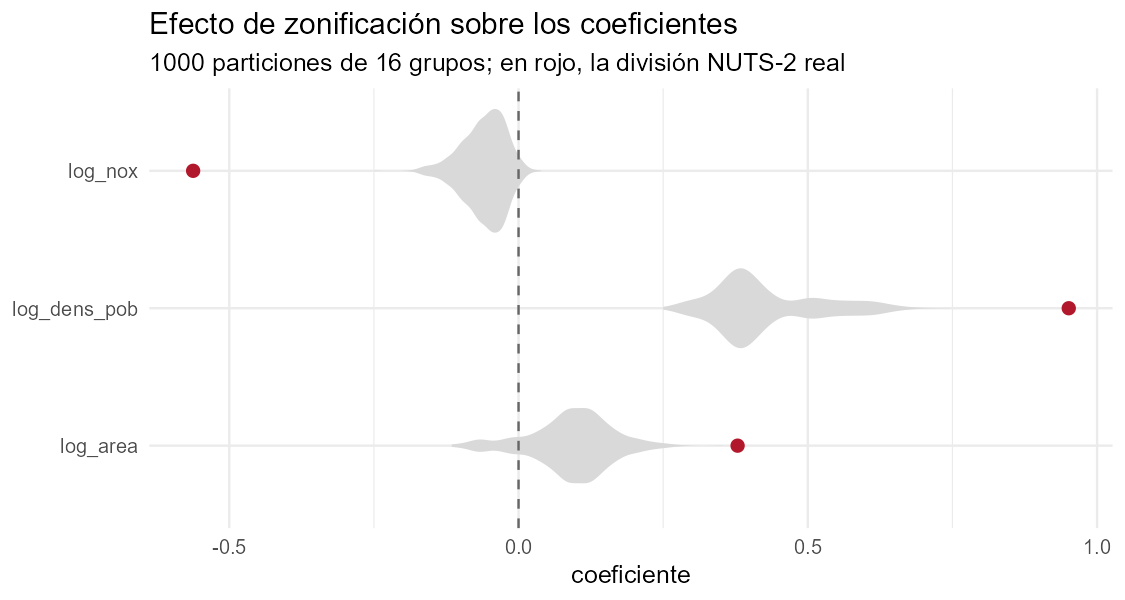
\includegraphics[width=\linewidth]{../output/figuras/43_maup_zonificacion.png}
\caption{Distribución de los coeficientes sobre \num{1000} zonificaciones
alternativas de \num{16} grupos. En rojo, el valor sobre la división
\textsc{nuts}-2 real.}
\label{fig:zonificacion}
\end{figure}

\subsection{Por qué desaparece}

La explicación es geométrica y cuantificable. La provincia media española mide
\SI{9970}{\kilo\metre\squared}: un disco equivalente de \SI{113}{\kilo\metre}
de diámetro. Un radio de influencia de \SI{10}{\kilo\metre} cubre el
\SI{0.8}{\percent} de esa superficie. Agregar a \textsc{nuts}-3 promedia la
señal industrial contra dos órdenes de magnitud de territorio donde el
mecanismo no opera.

La urbanización sobrevive a la agregación porque \emph{opera} a escala
provincial; la industria no. La diferencia no está en la intensidad del
mecanismo sino en su alcance espacial (figura~\ref{fig:escala}).

\begin{figure}[t]
\centering
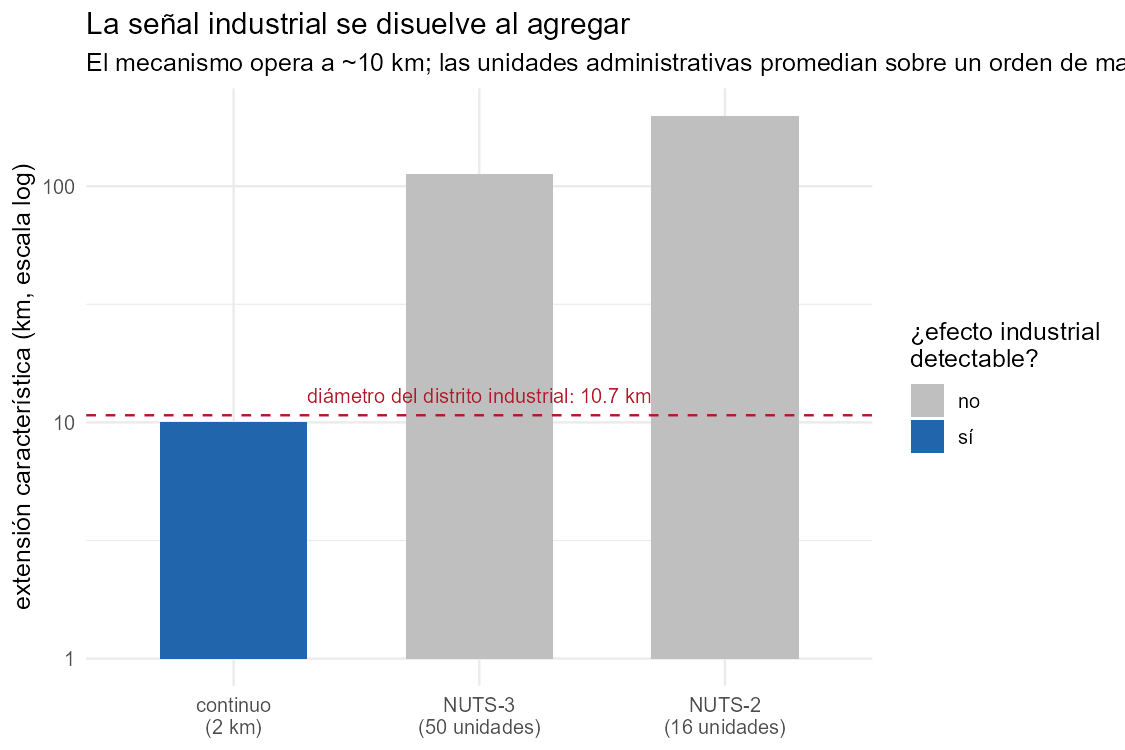
\includegraphics[width=\linewidth]{../output/figuras/50_curva_escala.png}
\caption{Extensión característica de cada soporte espacial frente al diámetro
del distrito industrial estimado (línea discontinua).}
\label{fig:escala}
\end{figure}

\subsection{Descomposición de varianza y cota del efecto}

La descomposición LMG \citep{gromping2006} del modelo de tres predictores
asigna el \SI{84.5}{\percent} del $R^2$ a la densidad de población, el
\SI{10.8}{\percent} al área y el \SI{4.9}{\percent} a las emisiones.

Con el conjunto completo de covariables, la varianza única total es solo el
\SI{19.7}{\percent} del $R^2$; el \SI{80.3}{\percent} restante es compartida
entre bloques y no atribuible a ningún mecanismo por separado. Este reparto es
en sí un resultado: a escala provincial los mecanismos son estadísticamente
inseparables porque la industria se ubica donde hay ciudades, puertos y
autopistas, que son las mismas variables que generan \ce{NO2} de tráfico.

Por último, el resultado más informativo del modelo areal no es un $p$-valor
sino una cota. El intervalo de confianza al \SI{95}{\percent} del coeficiente
industrial es $[\num{-0.1006}, \num{0.0617}]$; recorriendo todo el rango
observado de emisiones, el efecto máximo compatible con los datos es
\SI{0.956}{\ugm}, el \SI{22.3}{\percent} de la media areal nacional
(\SI{4.28}{\ugm}). No es que ignoremos si la industria influye: sabemos que no
puede influir más que eso.

\subsection{Implicaciones para la gestión}

La ponderación dasimétrica por población eleva la exposición estimada de
Madrid de \SI{7.52}{\ugm} a \SI{15.01}{\ugm} y la de Barcelona de
\SI{6.64}{\ugm} a \SI{14.21}{\ugm}. Tres provincias superan el
\SI{10}{\percent} de población por encima de \SI{20}{\ugm}: Madrid
(\SI{37.3}{\percent}), Barcelona (\SI{30.6}{\percent}) y Bizkaia
(\SI{22.7}{\percent}).

El contraste que cierra el análisis: el \SI{43.3}{\percent} de las estaciones
de tráfico superan hoy los \SI{20}{\ugm}, frente al \SI{0.16}{\percent} de la
superficie de fondo. España cumple con holgura la directiva vigente y tiene
margen frente al umbral de 2030 \citep{directiva2024}, pero está lejos de la
recomendación de la OMS \citep{who2021}, y el problema reside en una escala
por debajo de la que este trabajo puede resolver.

% =============================================================================
\section{Discusión y limitaciones}

\paragraph{Qué aporta cada rama.} Ninguna de las tres ramas responde la
pregunta por sí sola. La geoestadística proporciona concentración en puntos no
muestreados con incertidumbre propagada, y separa campo de fondo de recargo
microescala; el modelo areal no puede recuperar el interior de la unidad y el
proceso puntual no observa concentraciones. El proceso puntual establece dónde
se ubican las fuentes y por qué, y detecta distritos tras condicionar en
covariables; la geoestadística trata las fuentes como covariable dada, y el
modelo areal no distingue veinte instalaciones agrupadas de veinte dispersas.
El modelo areal produce cifras sobre la unidad en que se legisla y pondera por
población. Y la comparación entre escalas exige dos ramas metodológicamente
independientes: es el único resultado que ninguna produce sola.

\paragraph{Limitaciones.} En orden de importancia:

\emph{(i)} El umbral de declaración E-PRTR es de \SI{100}{\tonne} anuales de \ce{NOx}; la marca mínima observada es \SI{102}{\tonne}. El patrón representa
grandes emisores, no toda fuente industrial.

\emph{(ii)} Canarias, con el \SI{24}{\percent} del \ce{NOx} industrial
español, queda fuera del dominio. Nuestras conclusiones aplican a la España
peninsular y balear, no al conjunto del Estado.

\emph{(iii)} La superficie modela \ce{NO2} de fondo, no exposición máxima. Los
picos de tráfico ocurren por debajo de la resolución de \SI{2}{\kilo\metre}:
el análisis señala su propio punto ciego.

\emph{(iv)} La clase 121 de CORINE mezcla industria con comercio y logística,
por lo que está casi colineal con urbanización. La señal industrial limpia es
el patrón E-PRTR, no la cobertura del suelo.

\emph{(v)} Los pesos dasimétricos no se escalan por población provincial: las
medias dentro de cada provincia son correctas, el agregado nacional está
sesgado.

\emph{(vi)} Las envolventes de Monte Carlo se calculan con $\lambda$ fijada de
los propios datos, lo que hace el contraste ligeramente anticonservador.

\emph{(vii)} Con \num{50} unidades areales, el modelo de la
ecuación~\eqref{eq:areal} tiene poca potencia; el diagnóstico de influyentes
lo confirma. La cota del efecto industrial debe leerse teniendo esto presente.

\emph{(viii)} El variograma gaussiano ganó por poco al esférico, e implica
variación por debajo de la menor distancia entre estaciones, un supuesto poco
creíble en calidad del aire.

\paragraph{Trabajo futuro.} Una formulación jerárquica bayesiana con SPDE
\citep{lindgren2011} permitiría propagar la incertidumbre de la superficie
predicha hacia el modelo areal, en lugar de tratarla como dato. La extensión
temporal a la serie 2019--2023 permitiría explotar el cierre de instalaciones
como cuasiexperimento.

% =============================================================================
\section{Conclusiones}

Dos estimaciones metodológicamente independientes ---una que solo observa
coordenadas de instalaciones, otra que observa concentraciones--- sitúan la
escala de la influencia industrial sobre el \ce{NO2} de fondo en España en
torno a \SI{10}{\kilo\metre}, con una razón entre ambas de \num{0.93}. La
unidad de influencia es el distrito industrial, no la instalación aislada.

Ese mismo efecto es indetectable a escala provincial, y la desaparición no
obedece a falta de potencia sino a que la unidad de análisis promedia la señal
sobre un territorio dos órdenes de magnitud mayor que su alcance. El
resultado resiste cuatro intentos de refutación y \num{1000} zonificaciones
alternativas.

Metodológicamente, el trabajo ilustra que el problema de la unidad espacial
modificable puede pasar de advertencia genérica a diagnóstico cuantitativo
cuando se dispone de una escala de referencia estimada externamente. Sin la
rama de procesos puntuales, el resultado nulo areal sería indistinguible de
una ausencia real de efecto.

% =============================================================================
\section*{Disponibilidad y reproducibilidad}

El código completo, los guiones de descarga y las instrucciones de ejecución
están disponibles en \url{https://github.com/randyfernandezp/no2-espana}. El
repositorio incluye un guion de verificación de integridad
(\texttt{R/99\_verificar.R}) que comprueba invariantes de conservación y
frescura de los ficheros derivados.

\bibliography{refs}

\end{document}
